\documentclass[11pt, a4paper, twocolumn]{jsarticle}
%
\usepackage{amsmath,amssymb}
\usepackage{bm}
\usepackage{graphicx}
\usepackage{ascmac}
\usepackage{subfigure}
\usepackage{multicol}
\usepackage{setspace}
\usepackage{mediabb}
\usepackage{float}
\usepackage{latexsym}
\usepackage{url}
\usepackage{cite}
\usepackage{layout}
\usepackage[top=30truemm,bottom=30truemm,left=16truemm,right=16truemm]{geometry}
%

\setlength{\textwidth}{178truemm}
\setlength{\textheight}{39\baselineskip}
\addtolength{\textheight}{\topskip}
\setlength{\voffset}{-0.5in}
\setlength{\headsep}{0.3in}
%
\renewcommand{\baselinestretch}{0.8}
\renewcommand{\figurename}{図}
\renewcommand{\tablename}{表}
\renewcommand{\headfont}{\bfseries}

\pagestyle{empty}

\begin{document}
% \twocolumn[
% \begin{screen}
% \begin{flushleft}
% aa\hspace{\fill}yyyy/mm/dd
% \end{flushleft}
% \begin{center}
% {\Large  和文タイトル  \\
% 英文タイトル}
% \end{center}
% \begin{flushleft}
% 工学系研究科 電気系工学専攻 関谷研究室\hspace{\fill}修士課程1年 37-136482 藤居 翔吾
% \end{flushleft}
% \end{screen}
% ]

\twocolumn[
\vspace{1.5cm}
\begin{center}
{\Large データセンター環境におけるショートフロー通信改善手法の一提案}\\
\vspace{1em}
{\large $藤居\;翔吾^{\dagger}$ \hspace{1.0cm}$田崎\;創^{\ddagger}$ \hspace{1.0cm}
$関谷\;勇司^{\ddagger}$}\\
${}^{\dagger}$東京大学大学院工学系研究科\\
${}^{\ddagger}$東京大学情報基盤センター \\
\end{center}
\begin{quotation}
\begin{spacing}{0.6}
{\footnotesize クラウド型のサービスの性質により, 今日のデータセンターではデータセンター内のトラフィックが増大しており,
複数の経路を持つネットワーク環境を応用して, 通信性能向上を目指す取り組みがされている.
しかし, 様々なニーズを抱えるトラフィックが混在している中で, レイテンシ志向なサイズの小さいフローに対し,
既存のMPTCP実装では性能を劣化させる問題が報告されている.
そこで本論文では, この問題に対し, 並列分散処理アプリケーションが稼働しているクラスターPCのトラフィックを観測する事で, 単一NIC(Network
Interface Card)への通信集中によるキュー負荷の影響がある事を示し,
それぞれのノードが複数のキューを持つネットワーク環境において,
通信経路を切り替えることによりキューの負荷を分散させる手法を提案した.
この手法による効果について, 中継スイッチとエンドノードに対してスループット, フロー完結時間の二つのメトリックを用いた予備検証を行い,
改善手法が与える影響を考察する.
}
\end{spacing}
\end{quotation}

\begin{center}
{\Large A proposal method for shortflow traffic in datacenter network }\\
\vspace{1em}
{\large ${\rm Shogo\;Fujii^{\dagger}}$
\hspace{1.0cm}${\rm Hajime\;Tazaki^{\ddagger}}$ \hspace{1.0cm}
${\rm Yuji\;Sekiya^{\ddagger}}$}\\
${}^{\dagger}$The University of Tokyo, Graduate School of Engineering\\
${}^{\ddagger}$The University of Tokyo, Information Technology
Center \\
\end{center}
\begin{quotation}
\begin{spacing}{0.6}
{\footnotesize
As increasing the amount of traffic in a datacenter by cloud service, the
effective network for utilization of massive computer clusters has been studied.
Recently, Multipath TCP(MPTCP) has been tackled this problem.
MPTCP can achieve the effective consumptions of the resources with multipath,
but a researcher reported MPTCP causes the delay of flow completion for short
flows.
In this paper, I presented measurements of the distribute processing cluster PCs
and reveal impairment mechanisms that lead to that latencies, rooted in single
NIC(Network Interface Card) with intensive load traffic, and proposed the method balancing
the load of queue for multiple queue, in such a MPTCP datacenter model.
I verified the effect of the method for switch and end-node with two metrics,
FCT(Flow completion time) of short flows and throughput of backgroung flows,
and considered the effects of the load balancing method as preliminary
experiment. }
\end{spacing}
\end{quotation}

\vspace{1.5cm}
]


\section{まえがき}
\label{sec:introduction}
今日の一般家庭のインターネット接続環境がギガビット級の速度に達しようとしている中, 多様の端末がインターネットに接続できるようになり,
大量かつ多種多様なデータの取得が可能となった.
特にトラフィックデータ量の増加傾向は顕著で, 18$\sim$24ヶ月単位で総データ容量が2倍になるという予測がされている~\cite{IBM_rep}.
またFacebookでは, 300ペタバイト以上のデータ量を保有しており, 1日あたりに1ペタバイトのデータを解析している~\cite{presto}.
このように近年では, ビッグデータの活用が着目され, 例えばウェブ検索エンジン, SNS(Social Networking
Service)などのデータセンターを用いたクラウド型サービスにおいて, リアルタイムに近いレスポンスを返すような場面で使われ始めている.
そのようなクラウドサービスには近年, より高いユーザーエクスペリエンスが要求されており,
Amazonでは100[ms]の遅延により売り上げが1\%下がる, といった報告~\cite{amazon}があるように,
例えばeコマースサイトでの商品購入や,
インターネット広告のコンバージョンのようなユーザの意思決定へのレスポンス遅延の影響は深刻な問題である~\cite{customer_impact}.
そのため, 大規模データをより高速に処理することが求められており, データセンターではサーバ運用台数が増加の一途を辿っている.
そうした中で, 可用性, 計算性能, 低コストの三つの要件がデータセンターの抱える課題となっている~\cite{requirement}.
特に計算性能について, 大量の計算機資源から最大限の性能を引き出すためには,
従来の仕組みではデータセンター内トラフィックに対して一部の資源にトラフィックが集中する問題に対応できないため,
計算機資源を有効活用するための研究が盛んに行われている\cite{mapreduce, fattree,
dctcp, improving, detail, p_fab}.
そのようなスケーラビリティ拡大には, ネットワークトポロジー, アプリケーション, プロトコルに対する三つのアプローチがある.

ネットワークトポロジーを改良するアプローチでは, 従来の単純な階層構造では,
データセンター内で発生するトラフィックに対して帯域が最大限割り当てられない~\cite{fattree}.
そのため,
近年ではそのようなトラフィックに対してスイッチを多段に構成することで帯域を有効利用するトポロジーが提案されており,
マルチパス環境を実現している~\cite{fattree}.

大量データの処理速度を改良するアプローチでは,
並列分散処理のためにpartition-aggregate計算モデルが提案されている.
MapReduce~\cite{mapreduce}等の並列分散処理フレームワークは,
この計算モデルに従っており, 今日の大規模クラウドサービスにおいては, 必要不可欠である.

プロトコルを改良するアプローチでは,
従来のTCPを拡張したMultipath TCP
(MPTCP)~\cite{mptcp}をデータセンターネットワークに用いる提案がされている~\cite{fattree}.
MPTCPを用いることにより, OSの制御によって複数のNIC(Network Interface Card), 複数の経路を同時に利用し,
スループットを向上させることが期待されている.

しかし, 並列分散処理フレームワークを用いることで発生する, 大量のフローサイズの小さいクエリーフローが遅延を引き起こし,
MPTCPを用いたマルチパス環境で, さらなる性能障害を引き起こす問題が報告された~\cite{improving, rtt}.

このような背景から,
データセンターにおけるマルチパスネットワーク環境でのショートフロー遅延の問題は並列分散処理アプリケーションの性能の面で深刻な問題である.
そこで本論文では, データセンターにおけるショートフロー遅延の問題解消のため, 二つの検証を行った.

一つは, 実環境の並列分散処理アプリケーションが稼働しているクラスターPCを用いて, 実トラフィックの観測, 解析を行った.
クラスターPCの定常状態時と並列分散処理を実行している時の二種類のトラフィックを解析することで,
並列分散処理アプリケーションが生成するトラフィックパターンの特徴および, 汎用的なネットワーク機器を用いた低コストなデータセンターにおけるショートフロー遅延が生じる背景について, ボトルネックとなりうるネットワーク環境を検討し, その原因を示した.

二つ目は, マルチパスネットワーク環境における, 複数のNIC, 複数の経路を利用した経路切り替えによる改善手法を提案する.
これは, 複数の経路を利用し, スイッチやエンドノードの持つ複数のキューへと負荷を分散させることで, 単一のキューへ負荷が集中することで生じていたキューイングやプロトコル処理の遅延を抑える事ができる, という仮定に基づいた提案手法である.
この手法により, 並列分散処理におけるショートフローのような低レイテンシが求められる通信においては, 他のフローの影響を受けずにすぐに割込み処理が行われ,
受信処理のCPU負荷の分散を期待しており, その効果を実機を用いた実験で検証した.
そして今後の課題として, 経路切り替えのアルゴリズム検討する.


\section{関連研究}
\label{sec:related}
本章では, これまでに報告されている複数経路利用によるフロー完結時間短縮化技術について簡潔に述べ, その優位性や問題点を示す.

2010年にAlizadehらによって, データセンターネットワーク特有のトラフィックパターンに特化して,
パラメータを決定するアルゴリズムが提案された~\cite{dctcp}.
データセンター特有のバースト性のあるトラフィックが引き起こす問題点として, キューの生成によるキューイング遅延, キュー溢れによるパケットロス,
スイッチのバッファに掛かる負荷がある.
これらの問題に対し, 経由するスイッチにおいて, ECN(Explicit Congestion Notification)によってエンドノードに輻輳を通知し,
キューの大部分が占有される前にウィンドウサイズを動的に変化させ, キューサイズを小さく保つアルゴリズムによって,
大部分のキューの伝送時間を短縮することを可能にした.
しかし, 大規模計算資源を想定したトポロジーにおける検証がされておらず, また各ネットワークデバイスに細かなチューニングを必要とするため,
大規模データセンターでは運用面での問題がある.
さらに, サイズの大きいフローの割合の大きいトラフィックの中では, その影響によりウィンドウサイズを小さくする制御が働くため,
サイズの小さいフローの完結時間への効果が小さい, と報告されている~\cite{p_fab}.

2011年にCostinらによって, MPTCPを用いたデータセンターネットワークモデルが提案された~\cite{improving}.
近年の大規模計算資源を有効活用するために提案されたネットワークトポロジーでは,
高性能なデバイスや特殊な機器を必要とせず, 汎用的なネットワーク機器のみを用いてデータセンター内のエンドノード同士の通信に経路が複数用意されている.
既存の取り組みでは, 通信に使わない経路をセカンダリ経路として利用することで, 耐障害性を持たせていたのに対し, 提案されたデータセンターモデルでは,
MPTCPを用い複数経路を同時に利用する事で, 耐障害性を保ちながら, 帯域を最大限利用する事を可能にした.
また, 様々なトポロジーにMPTCPを適用することで, 従来のTCPよりも高いスループットが出せることを示した.
しかし, MPTCPとSingle path-TCPが混在する環境において, Single
path-TCPで行われるサイズの小さいフロー($\leq70KB$)のフロー完結時間に着目すると, 従来のSingle
path-TCPのみのネットワーク環境よりも時間がかかるという問題点があった.

2012年にZarsらによって, 複数レイヤー間でトラフィックを監視し,
しきい値を設定することによるフロー完結時間の短縮化技術を提案した~\cite{detail}.
今日のデータセンター内ネットワークのような, サイズの異なるフローが混在するネットワークにおいては, サイズが小さいフローがサイズの大きいフローに圧迫され,
伝送遅延が大きくなる問題があったが, この提案手法では, データリンク層からアプリケーション層までの各層が,
相互にトラフィックを監視する機能をスイッチに実装し, 優先度をつけ, バッファサイズを調整することで, フロー完結時間の劣化を抑えることを可能にした.
しかし, 実験ではClick~\cite{click}を用いて実装を行っており, 現実世界での全てのネットワーク機器の置き換えが必要となるので, 実現は難しい.

以上で述べたことをまとめると, 近年のデータセンターネットワークに対して, 以下のような要件が考えられる.
\begin{itemize}
  \item 大規模計算機を有効活用するトポロジーの利用
  \item 分散処理の際に発生する大量のサイズの小さいフローの送信時間の短縮
  \item 特殊な実装やデバイスを用いず, シームレスな運用の実現
\end{itemize}

\section{データセンターネットワーク}
\label{sec:datacenter}
本章では, データセンターネットワーク環境を構成する技術に関して, その概要を述べる.
\subsection{マルチパス環境を実現するネットワークトポロジー}
\label{sec:topology}

従来のデータセンターモデルでは, HostがEdgeスイッチにつながり,
これらのスイッチがAggregationスイッチに集約され,
coreスイッチに接続するといったように, 階層的に二分木トポロジーを形成していた~\cite{fattree}.
このような単純な階層構造を持つトポロジーは, トラフィックの大部分がデータセンター外の通信には有効であった.
しかし, 今日のようなデータセンター内で生じるトラフィックが大半を占める場合, 上の階層にある広帯域の経路を使わない通信が増え, 帯域の割当が不適切となる.
近年の研究~\cite{fattree}では, トラフィックがデータセンター内に集中した時の問題を, 物理的なアプローチとして,
トポロジーを工夫する事で解消を試みている.

図\ref{fig:fattree}のように, FatTree~\cite{fattree}では, Coreスイッチを複数用いる事で,
物理パスの最大帯域を供給する.
また, 比較的狭い帯域の経路と汎用的な性能のスイッチを多数用い, データセンター内のエンドノード同士の通信で複数の経路を実現する事で, 冗長化,
ネットワーク資源の効率的な利用, 低コストを実現している.

しかしこのような密な配置により, 複数の経路が形成され, ルーティングをどのように決定すべきかという問題も生じる事となる~\cite{improving}.
例えば図\ref{fig:fattree}のFatTreeトポロジーでは, 4通りの経路が考えられる.
これら複数の経路をリンクエラー時の冗長性を持たせる目的だけでなく, 性能向上に活用することが求められており, MPTCPではスループットに対し,
性能向上を実現する\cite{improving}.
 \begin{figure}[h]
    \begin{center}
    \includegraphics[autoebb, width=210pt]{./img/fattree_topology.pdf}
    \caption{Fattree トポロジー}
    \label{fig:fattree}
    \end{center}
\end{figure}

\subsection{トラフィックシナリオ}
\label{sec:traffic_scenario}
大量の計算機資源を有効活用するためには,
並列分散処理フレームワークを用いられ, 一般的にpartition-aggregate構造をとる.
並列分散処理フレームワークでは, 多数の処理ノードと分散処理の制御をする管理ノードから構成されており, 管理ノードからクエリーが発行され,
処理ノードがそれを受け取り,レスポンスを返す.
このとき, トラフィックパターンが  (1){\it Query traffic}, (2){\it Short message
traffic}, (3){\it Backgroung traffic}の3つに分類される~\cite{dctcp}.

{\bf Query traffic. }Query trafficとは, 大規模計算処理を分割して並列処理を開始する際に,
aggregatorノードから処理ノードへ具体的な処理を割り当てるためのトラフィックである.
Query trafficの特徴は, 非常に小さいフローサイズ(2KB$\sim$20KB)で,
フローの役割上, 処理全体の遅延に非常に強く影響を及ぼす事である.
そのため, アプリケーション性能を考慮すると, 低レイテンシでの通信が求められている.
また並列分散処理システムの構成上, Query trafficはms$\sim \mu$s単位で生成され,
バースト性があるといえる~\cite{dctcp}.

{\bf Short message traffic. } Short message trafficとは,
処理ノードの動作を制御するためのトラフィックである.
Short message trafficの特徴は, フローサイズは50KB$\sim$1MBで, Query
trafficと同様に処理全体の遅延に影響を及ぼすという事である.
しかし, Querry trafficほどのフロー数は生成されず, 生成間隔も秒単位である.

{\bf Backgroung traffic. }Backgroung trafficは,
各処理ノードへ更新データを送信するトラフィックである.
Backgroung trafficの特徴は,フローサイズが1MB$\sim$50MBと大きいことにある.
さらに, その生成間隔は大きい.
また, Backgroung trafficでの更新データは, 処理精度の向上に寄与するが, 処理に必須ではないので,
処理全体の遅延にはつながらない.

つまり, 分散処理開始時に生成されるQuery trafficが遅延すると,
処理全体に対し遅延を引き起こすので, Query trafficを含むショートフローのフロー完結時間は極めて重要なメトリックである.

また, Alizadehらは, 実際のデータセンターのトラフィックでは, レイテンシ志向なショートフローとスループット志向なロングフロー,
そしてバースト性のあるQuery trafficが混在していると報告している.
さらに, Background trafficのフロー数自体は少ないが,
全体のトラフィック量の大部分がBackgroung trafficによって占められているという特徴がある~\cite{traffic}.

\subsection{実トラフィック解析}
\label{sec:traffic_character}
この節では, クラウドサービスを想定したトラフィックの一例として並列分散処理アプリケーションを用いた二種類のトラフィックの測定結果を示す.
測定結果からトラフィックの特徴を示す事で, 従来のTCPで構成されたクラスターの抱えるボトルネックと複数のキュー,
複数の経路を持つマルチパス環境におけるデータセンターモデルの利点をそれぞれ示し, 提案手法の需要を裏付けるものとなる.

測定環境には, 管理ノード1台(Master), 処理ノード10台の計11台のクラスターPCを用いた.
管理ノードは10GbpsイーサネットリンクでTop of Rack(ToR)スイッチに接続されている.

このクラスターPCでPresto~\cite{presto}によりインタラクティブなレスポンスを返す, 分散SQLデータベースを実現しており,
\S \ref{sec:traffic_scenario}で示した三種類のトラフィックが混在している.
トラフィックの測定には, 管理ノードのインターフェースを用いて, tcpdump\cite{tcpdump}によるパケットレベルの測定を行った.

{\bf 定常状態: }
管理ノードに対し, ジョブ命令を一切与えていない中で約10時間程度トラフィックを測定した.
図\ref{fig:constant}に定常時のフローサイズの確率分布を示す.
この分布が示すように, ショートフローの数が全体のトラフィックの大部分を占めている.
実際, 80\%以上のフローが10KB以下であった.
一方で, 通信量に着目すると, フロー数は比較的少ないがフローサイズの大きいトラフィックが大半を占めている.

次に, 図\ref{fig:constant_cdf}に管理ノードへのトラフィックの影響を示す.
この分布が示すように, 各処理ノードから管理ノードへのトラフィックの割合が大きく, それぞれフローサイズも大きい.
一方で, 管理ノードから各処理ノードへのトラフィックについては, 比較的フローサイズの小さいトラフィックの割合が大きい.

さらに, 図\ref{fig:constant_conc}に時間毎の同時接続数の分布を示す.
この分布が示すように, 各処理ノードから管理ノードへのトラフィックの同時接続数が多く, 積極的に通信が行われている.
また, 短い通信時間でスパイク性のある中で, 長時間通信を行うフローが固定的に存在している.

\begin{figure}[t]
    \begin{center}
    \includegraphics[autoebb, width=210pt]{./img/constant.pdf}
    \caption{Prestoクラスタの定常時のトラフィック分布}
    \label{fig:constant}
    \end{center}
\end{figure}

\begin{figure}[t]
    \begin{center}
    \includegraphics[autoebb, width=210pt]{./img/constant_cdf.pdf}
    \caption{管理ノードから見た定常時のトラフィック累積分布}
    \label{fig:constant_cdf}
    \end{center}
\end{figure}

\begin{figure}[t]
    \begin{center}
    \includegraphics[autoebb, width=210pt]{./img/constant_conc.pdf}
    \caption{定常時トラフィック:同時接続数の分布}
    \label{fig:constant_conc}
    \end{center}
\end{figure}

{\bf 並列分散処理実行時: }
管理ノードに対し, 約1分間程度で完了するSQLジョブを与えた中でジョブが完遂するまでの間トラフィック測定を行った.
SQLジョブには, ``$select * from \, \$テーブル where \, \$条件$"を実行し,
全ての処理ノードがジョブを与えられるようにした.
図\ref{fig:job}にジョブ実行時のフローサイズの確率分布を示す.
この分布が示すように, ショートフローの数が全体のトラフィックの大半を占めるが, 定常状態と比べると,
全体的にフローサイズ大きいトラフィックが増えている.
実際, 80\%以上のフローが110KB以下であったように, ショートフローの割合が小さくなった.
同様に通信量に着目すると, フロー数は比較的少ないがフローサイズの大きいトラフィックが大半を占めるという事が分かる.

次に, 図\ref{fig:job_cdf}に管理ノードへのトラフィックの影響を示す.
この分布が示すように, 各処理ノードから管理ノードへのトラフィックの割合が大きく, フローサイズは小さいものが多いことが分かる.
しかし, 図\ref{fig:constant_cdf}の定常時のトラフィックと比べると,
管理ノードから各処理ノードへのトラフィックの割合が大きくなっている.

次に, 図\ref{fig:job_conc}に時間毎の同時接続数の分布を示す.
この分布が示すように, ジョブ実行中は全体的にフローの数は増え, とりわけ管理ノードから各処理ノードへのトラフィックの割合が大きくなっている.
さらに, ジョブ終了後も同時接続数が大きく変化していないことから, 長時間通信を行うフローが固定的に存在している.
また, 各処理ノードから管理ノードへのトラフィックに着目すると, ジョブ開始時に接続数が大きく増えている事から, バースト性があるトラフィックであるといえる.

\begin{figure}[t]
    \begin{center}
    \includegraphics[autoebb, width=210pt]{./img/job.pdf}
    \caption{Prestoクラスタのジョブ実行時のトラフィック分布}
    \label{fig:job}
    \end{center}
\end{figure}

\begin{figure}[t]
    \begin{center}
    \includegraphics[autoebb, width=210pt]{./img/job_cdf.pdf}
    \caption{管理ノードから見たジョブ実行時のトラフィック累積分布}
    \label{fig:job_cdf}
    \end{center}
\end{figure}

\begin{figure}[t]
    \begin{center}
    \includegraphics[autoebb, width=210pt]{./img/job_conc.pdf}
    \caption{ジョブ実行時トラフィック:同時接続数の分布}
    \label{fig:job_conc}
    \end{center}
\end{figure}

これらの分布から, クラウド型サービスを想定したトラフィックの一例として並列分散処理アプリケーションを実行した際の特徴として以下の事が述べられる.
\begin{itemize}
  \item 定常時もジョブ実行時も同様に, 管理ノードへ送信されるトラフィック量は多い
  \item 長い時間通信を行うフローが固定的に存在している
  \item ジョブ実行時の処理ノードから管理ノードへのトラフィックには, フローサイズも小さく, バースト性がある
\end{itemize}

これらの特徴から, 管理ノードへのトラフィックが集中する問題, ショートフローのバースト性の問題,
そして長時間通信を行うBackgroung trafficの問題が生じていると考えられる.
従って, 大きく二つの管理ノードに対するトラフィックパターンを検討する必要がある.
\begin{enumerate}
  \item ジョブ開始時のバースト性のあるショートフロートラフィック
  \item アプリケーション性能に直接影響しないBackgroung trafficが通信している中で,
  低レイテンシ通信が求められているショートフローの通信
\end{enumerate}


\section{提案手法}
\label{sec:proposed_method}
データセンターにおけるマルチパスネットワークの研究動向と, 並列分散処理アプリケーションが生成する特有のトラフィックパターンが引き起こす機能障害をふまえて,
改善手法の提案を提案する.

提案手法のきっかけとなったのは, MPTCPを用いたデータセンターネットワークモデルである\cite{improving}.
このネットワークモデルでは, 基本的にエンドノードは複数のNICを持ち, 一つのフローの通信でそれらを同時に利用することでスループットを向上させる.
このような複数経路の効率的利用には, IPベースのルーティングで実現しており, それぞれのエンドノードが持つIPアドレスのペアにより, 通信経路が決定する.
さらに, 現在のMPTCPの実装では, TCPの3ウェイ・ハンドシェイクでコネクションを確立した後の通信で, TCPオプション互いのIPアドレスを交換し,
新しいサブフローを形成するという仕組みになっている.
そのため, サイズの小さいフローの通信では, サブフローを形成するまでに通信が完結する.
また, 3ウェイ・ハンドシェイクでコネクションを確立するための最初のフローについては, クライアント側のIPアドレスの指定により通信経路が決定する.
以前の我々の解析では, このコネクション確立の際に遅延が生じることが分かっており\cite{mptcp_ana}, どの経路を利用するかによって,
性能性能が大きく変わる.
提案手法の目的は, 低レイテンシなネットワークを実現する事であり,
レイテンシ指向であるフローサイズの小さいショートフローをなるべく遅延を抑えながら通信を完結する事である.
こうした目的に対して, 提案手法では物理的に複数のキューを用意する事で, パケット処理の負荷を分散させる事ができると仮定し, その手法として,
複数のNICによるマルチパスネットワーク環境でのトラフィック制御がある.

提案するトラフィック制御では, スイッチ, エンドノードに対して, それぞれのキューの混雑具合を考慮し, 経路を決定する.
本質的な狙いは, フローサイズによって通信時間が決まるということであり, 例えば, フローサイズの大きいバックグラウンドフローが長時間通信を行っている中で,
ショートフローが発生した場合, バックグラウンドフローが占有しているキューを避けた通信経路で通信時間を抑えるというシナリオを実現するものである.

したがって, フローが生成された直後は他のフローよりも優先的に通信が行われ, サイズの小さいフローであれば素早く通信を完結できる.
しかし, フローサイズが大きいスループット指向な通信である場合, レイテンシ指向な通信に対してリソースを無駄にする事となる.
そのため, ある一定の状況でショートフローではないと判断されたら, 優先度を下げて他のショートフローにリソースを割り当て直す制御が必要である.
具体的には, 例えばMPTCPの輻輳制御を用いて, ウィンドウサイズを小さくすることで, 実質的に通信途中で経路を切り替える等が考えられる.

しかし, アプリケーションの実装を変更しない限り, 通信開始時点で転送するデータ量を知ることはできないため,
ショートフローであるかどうかを判断する仕組みについては今後検討すべきである.



\subsection{キュー負荷分散}
\label{sec:load_balancing_mechanism}
提案するトラフィック制御では, 大きく3つのフェーズから構成されている. \\
{\bf (1)Initial phase: }
提案手法ではフロー生成時には最も優先度が高く通信することができる.
そこで, 通信開始時点でエンドノードと中継スイッチに対して, 最も混雑していない組み合わせを選択し, 通信経路を選択する.
経路を選ぶ際には, 利用率[bps], フロー数, キュー長等を用いる事が考えられる. \\
{\bf (2)Judging phase: }
次に, そのフローがショートフローであるかどうかを判断する.
その際, ショートフローでないと判断された場合には, 優先度が低い通信であると判断され, 別の経路での通信へと比重が変わる.
その際に用いるメトリックとしては, データ転送量, 通信占有時間等が考えられ, 判断のためのしきい値を設定する必要がある.

{\bf (3)Switching phase: }
提案手法ではMPTCPを用いて, 複数の経路を用いた通信が可能であると想定する.
Judging phaseにおいて, ショートフローでないと判断された時, 輻輳制御を用いてウィンドウサイズを更新し, 各経路の通信量を制御する.
具体的には, 最初に割り当てられた通信経路のウィンドウサイズを下げ, 他の経路を利用する制御を行うという事である.
ウィンドウサイズの決定には, その増減量を決定するパラメータを設定する.

\subsection{期待される効果}
\label{sec:expected_effect}
この提案手法により, エンドノード, スイッチに対して引き起こす性能障害の影響を緩和することができる.

{\bf スイッチ - 性能障害}\\
現在のスイッチ機器では複数のフローを多重に扱うための共有メモリを持つ.
そして共有メモリプールからMMU(Memory Management Unit)によって各インターフェースが利用できるメモリ量を動的に割り当てる事で,
複数の通信を公平に処理する事を目指す.
しかし, 比較的安価なスイッチでは制御できるメモリ量が制限されているため,
様々な性能障害を引き起こす~\cite{flexible}.

\subsubsection{Incast}
\label{subsec:incast}
図\ref{fig:impair}(a)に示すように, 短期間に一つのインターフェースへとフローが集中した場合, 用意されているバッファを使い果たし,
最悪の場合パケットロスを引き起こす.
これは, \S \ref{sec:traffic_scenario}で示したpartition-aggregate構造によるもので,
リクエストを受けた処理ノードが同期して一斉にレスポンスを返すことにより,
そのレスポンスを集約して受け取るノードが接続しているスイッチでのポートのキューサイズが大きくなり, 遅延, パケットロスを生じる.
% こうした問題に対して, アプリケーションレベルにおいては二つのアプローチがある.
% 一つは, レスポンスのサイズを意図的に小さくし, スイッチバッファの圧迫を抑えることである.
% もう一つは, それぞれのリクエストにジッタを混ぜる事で, レスポンスを同期させないことである~\cite{synchro}.
% さらに, パケットロスを生じた際へのアプローチとしては, $RTO_{min}$を小さくする事でパケットロスの影響を抑える事ができる.

\subsubsection{Queue buildup}
\label{subsec:queue}
\S \ref{sec:traffic_scenario}で示したように, 並列分散処理のレスポンスには直接影響しないBackgroung trafficは,
スイッチバッファにパケットロスを引き起こすほどの影響を及ぼし, そのポートがボトルネックとなる可能性がある.
図\ref{fig:impair}(b)に示すように, Backgroung trafficとQuery trafficが同じポートを利用する場合に,
サイズの大きいフローによるショートフローのキューイング遅延が生じる, Queue buildup問題がある.
このキューイング遅延の問題に対する唯一の解決策は, キューサイズをなるべく小さく保つことにより, キューに溜まったパケットを素早く排出することである.

\begin{figure}[h]
    \begin{center}
    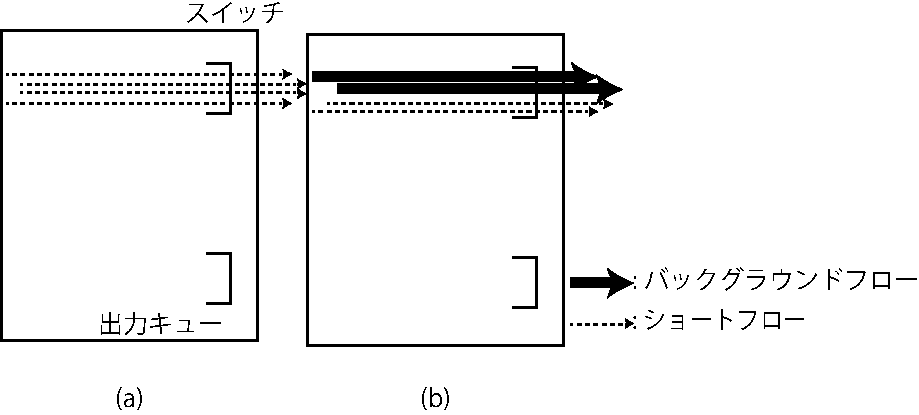
\includegraphics[autoebb, width=210pt]{./img/impairments.pdf}
    \caption{中継スイッチで引き起こすボトルネック}
    \label{fig:impair}
    \end{center}
\end{figure}


{\bf エンドノード - 性能障害}
今日のGbE(Gigabit Ethernet)通信において, 割込み処理は大きなボトルネック要因の一つである.
例えば, 1GbEにおいて64バイトフレームの最大受信可能数は, 毎秒約150万であり, 1パケット受信する度に割り込み処理を行っていては,
CPUリソースが枯渇する.
そのため, 割込み処理の回数を抑えることが必要であるが, その分レイテンシが上がる可能性があり, 互いのトレードオフを適切に対処し高い性能を得る必要がある.
また, 今日の多くのCPUはマルチコアであり, CPUリソースを効率的に利用する事が求められている.
\subsubsection{割込み処理}
パケット受信の際のNICによるハードウェア割込みは, 即座に受信処理を行う事ができ, キューイングの遅延を小さくする事ができる.
しかし, 割込み処理が増えれば, その分オーバヘッドが大きくなり, 結果的にOSの性能が劣化する.
割込み処理を扱う代表的な仕組みとして, ポーリング, interrupt coalescingがある.

ポーリングはNICの割り込みを使わず, タイマーを使って定期的にNICの受信キューを監視することで, 割り込み負荷を軽減するソフトウェア技術である.
しかし, NICでパケットを受けてから即座に処理できない為, 遅延が発生する場合がある.
現在のLinuxカーネルにおいては, NAPIにより, 通信量が多く高負荷時のみはポーリングが作用する~\cite{NAPI}

interrupt coalescingは, 複数のパケット, あるいは一定期間待ってからをまとめて一度で割り込ませる事で,
割込み回数を減らすハードウェア技術である.
しかし, ポーリングと同様, 即座に処理できない為, 遅延が発生する場合がある.

\subsubsection{プロトコル処理}
マルチコア環境においても基本的には一つのNICの受信処理は1つのCPUでしか行えない.
そのため, ハードウェアへのアプローチとして, 1つのNICに複数の受信キューを持たせて, 受信処理をそれぞれのCPUへ分散させている, Receive
Side Scaling(RSS)がある~\cite{RSS}.
しかし, 一般に複数受信キューを持ち, RSS機能があるNICは高価である\cite{intel}.
そのため, 一つしか受信キューを持たないNICであっても, 複数のCPUを分散させるソフトウェア技術として, RPS(Receive Packet
Sterring)がある~\cite{RPS}.
しかしRPSでは, プロトコル処理とアプリケーション処理のCPUが異なる場合が生じ, その問題を最適化したのがRFS(Receive Flow
Sterring)がある~\cite{RFS}.
これらの技術により, CPUの複数のコアをより効率良く利用する事ができる.

また, プロトコル処理やアプリケーションでの処理については, RFS等で複数のCPUへと分散させる事ができるが,
その際の割込み処理についてはオーバヘッドが生じる可能性がある.


\section{検証実験}
\label{sec:verification}
これまでの研究において報告されたMPTCPによるショートフロー性能劣化の問題~\cite{improving}を受け, その再現実験を行うことにより,
原因を解析し, 二つの要因を明らかにした~\cite{mptcp_ana}.
一つ目は, MPTCPはTCPよりも多くのトラフィックを排出し, より多くのNICインタフェースを利用する事で,
中継スイッチにおいてショートフローが利用するインタフェースと競合し, スイッチでの遅延, パケットロスが生じるということ
二つ目は, ショートフロートラフィックのバースト性の問題により, エンドノードで単一のNICに負荷が集中し, 受信処理の遅延が生じたということ
これらの結果を受け,
低レイテンシでの通信が求められるショートフローに対して, MPTCPによるバックグラウンドトラフィックが利用しているインタフェースを回避し,
比較的輻輳が起こっていない経路を適切に選ぶ事で,
単一キューへの通信負荷の問題は解消され, ショートフローのフロー完結時間(FCT)が改善できるのではないかと, 仮説を立てた.
この章では, 実機での実験を用いて, その仮説の検証,
また複数のキュー, 複数の経路を利用した経路切り替えによる改善手法の効果の検証を行う.
具体的には, 中継スイッチとエンドノードへのそれぞれの単一キューの負荷について, 複数のNICを用いて分散させ, その効果を検証する.

\subsection{実験環境}
{\bf (1)中継スイッチに対する負荷実験}\\
ネットワークトポロジーには, 2段で構成されたトポロジーを用いる.
図\ref{fig:topology_switch}に, 用いたトポロジーを示す.
ベンチマークトラフィックについては, 二つのペアに対してエンドノード同士の1対1通信を用いている.
一方のペアに対しては, シミュレーションを実行している間, 継続してデータ転送 (バックグラウンドトラフィック)を行う.
他方のペアに対しては, TCPによる70Kbyteのデータ転送(ショートフロー)を毎10msの一様生起させ,
転送完了までにがかかった時間FCT(Flow Completion Time)を計測している.
ショートフローのルーティングに関しては,
図\ref{fig:topology_switch}に示す3つのパターンを用いて中継スイッチへのインターフェースへの負荷の影響を検証する.


{\bf (2)エンドノードに対する負荷実験}\\
ネットワークトポロジーには, 二つのNICを持った二つエンドノード同士をL2スイッチを介してそれぞれのNIC毎に接続した.
図\ref{fig:topology_node}に, 用いたトポロジーを示す.
ルーティングに関しては, それぞれの対をなすNIC同士が通信を行う.
ベンチマークトラフィックについては, エンドノード同士の1対1通信を用い, ショートフローとバックグラウンドフローを通信させる.
バックグラウンドフローについては,
ショートフローが通信しているNICペアと同じものを使って共有して通信させるパターンとショートフローが通信しているNICペアとは異なるペアのNICを用いて通信を行うパターンの2パターンについて検証する.
ショートフローは, TCPによる70Kbyteのデータ転送を毎10ms一様生起させ, 転送完了までにがかかった時間を計測している.
バックグラウンドトラフィックは, シミュレーションを実行している間, 継続してデータ転送を行う.

以下に用いた機器の詳細を示す.
\begin{figure}[t]
    \begin{center}
    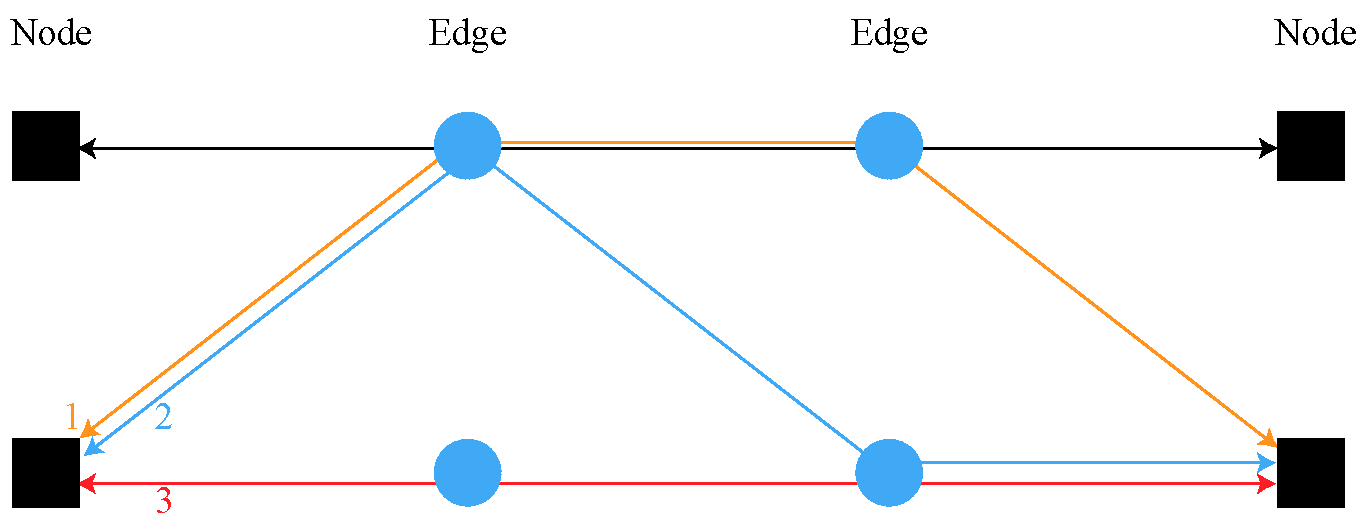
\includegraphics[autoebb, width=210pt]{./img/topology_ns3.pdf}
    \caption{中継スイッチへのNIC負荷実機実験トポロジー}
    \label{fig:topology_switch}
    \end{center}
\end{figure}

\begin{figure}[t]
    \begin{center}
    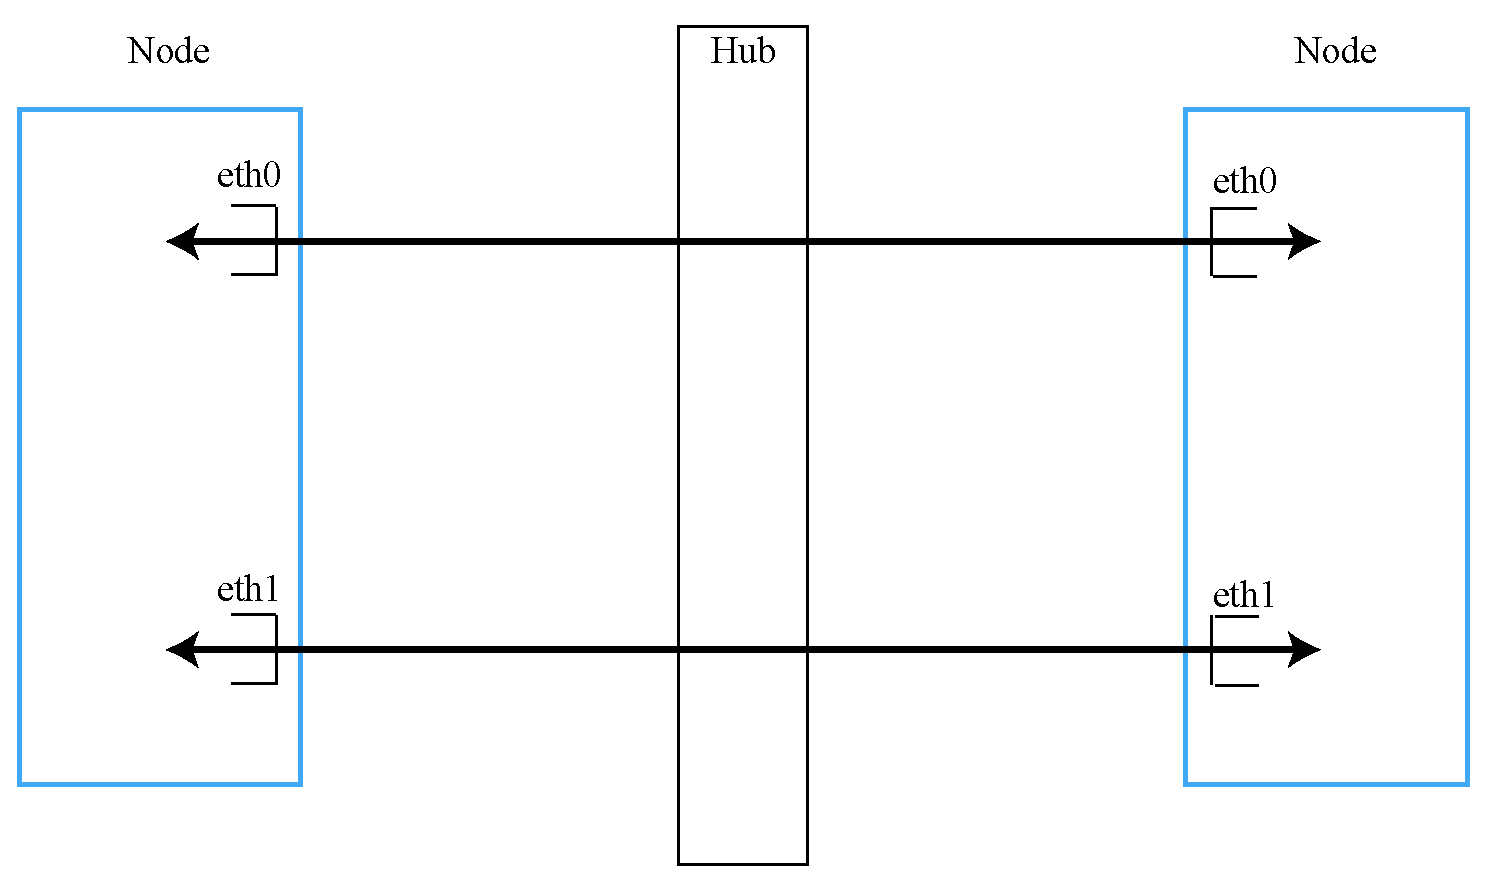
\includegraphics[autoebb, width=210pt]{./img/topology_real.pdf}
    \caption{エンドノードへのNIC負荷実機実験トポロジー}
    \label{fig:topology_node}
    \end{center}
\end{figure}

\begin{table}[h]
\begin{center}
\footnotesize
\begin{tabular}{c|c}
\hline
項目 & スペック \\ \hline \hline
OS & Linux 3.13.0 \\
CPU & Intel Xeon CPU L3426 \\
メモリー & 4GByte \\
NIC対応ドライバ & e1000 \\
スイッチ-実験1 & Catalyst 2940(100T) \\
スイッチ-実験2 & GS905L V2(1000T) \\
\hline
\end{tabular}
\caption{実験環境パラメータ}
\label{table:experiment_ver}
\end{center}
\end{table}

\subsection{実験結果}
{\bf (1)中継スイッチに対する負荷実験}\\
図\ref{fig:improve}に上記の実験環境での結果として, 70KBのショートフローのFCTとバックグラウンドフローの経路利用率を示す.
FCTの箱ひげ図の上端には, 95パーセンタイル値, 下端には最小値を用いている.
この結果から, ショートフローの通信が, 中継スイッチにおいて, バックグラウンドフローと経路およびインターフェースを共有した事による影響で,
FCTの分散が大きくなっている事が分かる.
一方で, 同じスイッチは利用する事になったもののインタフェースは共有しなかったトラフィックや,
バックグラウンドフローとは独立に通信を行っていたトラフィックに対しては, 何も影響がなかった.
これは, 単一NICキューに対して二つのトラフィックが集中したことによる遅延,
あるいは負荷分散の影響であると考えられる.
この影響からバックグラウンドフローに対しても, スループットが下がっている事が分かる.

これらの事から, アプリケーション性能に直接影響しないBackgroung trafficが通信している中で,
低レイテンシ通信が求められているショートフローの通信をする際, 中継スイッチでの利用するインタフェースが競合する場合,
単一のキューに対しトラフィックが集中する事で, 受信処理の割込みのオーバヘッドや, プロトコル処理の遅延の影響が生じたと考えられる.
よって, スイッチにおいて複数のキューに対し, トラフィックを分散させる事は, レイテンシ志向のショートフローに対しても,
スループット志向のバックグラウンドフローに対しても有効であるといえる.
\begin{figure}[h]
    \begin{center}
    \includegraphics[autoebb, width=195pt]{./img/switch_verif.pdf}
    \caption{中継スイッチに対する負荷実験での70kbベンチマークトラフィックに対するフロー完結時間とリンク利用率}
    \label{fig:improve}
    \end{center}
\end{figure}


{\bf (2)エンドノードに対する負荷実験}\\
図\ref{fig:real_exp0}に上記の実験環境での結果として,
70KBのショートフローのFCTとそれぞれの経路の利用率を示す.
FCTの箱ひげ図の上端には, 95パーセンタイル値, 下端には最小値を用いている.
この結果から, ショートフローの通信が, エンドノード間通信において, バックグラウンドフローと経路およびインターフェースを共有した事による影響で,
FCTの分散が大きくなっている事が分かる.
一方で, 経路, インタフェースは競合しなかったものの, バックグラウンドフローとショートフローが同時に通信を行ったことで,
FCT下位25\%のフローについては遅延が生じ, 分散が大きくなった.
これは, 単一NICに対して二つのトラフィックが集中したことによる負荷分散の効果が得られたが, プロトコル処理以降の部分で,
複数のフローが同時に通信を行った事に対するオーバヘッドが生じたと考えられる.
またバックグラウンドフローに着目すると, インターフェースを共有した場合においては,
ショートフローだけでなくバックグラウンドフローにも遅延が生じ, スループットが低下している.

これらの事から, アプリケーション性能に直接影響しないBackgroung trafficが通信している中で,
バースト性のあるショートフロートラフィックの通信をする際, エンドノードに対して, 利用するインタフェースが競合する場合,
単一のNICに対しトラフィックが集中する事で, 受信処理の割込みのオーバヘッドや, プロトコル処理の遅延の影響があると考えられる.
よって, エンドノードにおいて複数のNICに対し, トラフィックを分散させる事は, バースト性のあるショートフローに対しても,
スループット志向のバックグラウンドフローに対しても有効であるといえる.

\begin{figure}[h]
    \begin{center}
    \includegraphics[autoebb, width=210pt]{./img/real_eth0.pdf}
    \caption{エンドノードに対する負荷実験での70kbベンチマークトラフィックに対するフロー完結時間とリンク利用率}
    \label{fig:real_exp0}
    \end{center}
\end{figure}

\subsection{考察}
\label{sec:analysis}
これらの解析結果から, エンドノード, スイッチに対する機能障害が引き起こる要因について述べ, 今後の改善手法の検討を行う.\\
大量の計算機資源をいかに効率的に利用するか, という課題を今日のデータセンターは抱えており,
Hadoopのような並列分散処理アプリケーションを用いる事が一般的である.
今の並列分散処理システムがpartition-aggrigation構造である以上, 管理ノードや多段のクラスター構成であればアグリゲーターノードに対して, 処理ノードからのトラフィックが集中する問題は発生する.
その結果, Queue buildupやIncastのような単一キューへの負荷集中の問題が中継スイッチやエンドノードに対して生じ,
CPU性能を効率的に引き出せず, 並列分散処理の性能が劣化する.

こうした遅延の影響を軽減する為には, 混雑時の通信量を抑える制御を行う, あるいは混雑時にも空いているリソースを効率良く利用する事が必要である.
MPTCPによる存の計算機資源に対して複数NICを用いた性能向上を目指すように, 複数のフローからデータを受信する際に異なる物理ポートを利用する事で,
マルチコアを持つCPUの効率的な利用につなげられると期待している.
すなわち, 複数のキューに対して通信を分散させるように, トラフィックを制御する事で,
例えばレイテンシ志向なショートフローとスループット志向なバックグラウンドフローのような役割の異なるトラフィックを共存させ,
最適な通信の実現が可能であることを本論文では示した.
そのような物理的に複数のNICによりマルチキューが介在する汎用的な機器で構成されているネットワークの中で,
トラフィックをどのように制御するかという点については, スイッチやエンドノードのOSスタック等のどこで制御をするか, またどのようなアルゴリズムでそれを実現するかという事を検討する必要がある.

\section{あとがき}
\label{sec:conclude}
本論文では, データセンターにおけるショートフロー遅延の問題を解決する為に, 二つの検証を行った.

一つは, 実環境の並列分散処理アプリケーションが稼働しているクラスターPCを用いて, 実トラフィックの観測, 解析を行うことで,
ジョブ開始時のバースト性のあるショートフロートラフィックとBackgroung
trafficが通信している中でのショートフローの通信のトラフィックパターンが存在し,
汎用的なシングルキューNICを用いたネットワーク機器においては機能障害を引き起こす原因となることを示した.

二つ目は, MPTCPを用いたデータセンターネットワークモデルにおける, 複数のキュー, 複数の経路を利用した経路切り替えによる改善手法を提案した.
これは, 複数の経路を利用しスイッチやエンドノードの持つ複数のNICへと負荷を分散させることで, 単一のNICに負荷が集中することによる,
キューイングやプロトコル処理の遅延を抑える事ができる, という仮定に基づき, 提案する手法である.
この改善手法により, 他のフローの影響を受けずにすぐに割込み処理が行われ, レイテンシ志向なショートフローへの受信処理の遅延を軽減する事ができた.
また, スループット志向であるバックグラウンドフローに対しても, 通信性能を向上させる事ができた.

今後はネットワークの通信状況を考慮しながら, 優先して通信を行うショートフローの定義,
通信状況を示すパラメータ, しきい値の設定を通して, 通信経路を切り替えるアルゴリズムの検討を行う.

\begin{spacing}{0.7}
\footnotesize{
\begin{thebibliography}{99}% 文献数が10未満の時 {9}
\bibitem{IBM_rep}{日本アイ・ビー・エム株式会社. IBM 第1章
大容量データのバックアップ,
\url{http://www-06.ibm.com/systems/jp/storage/column/backup/01.html}}
\bibitem{amazon}{Jim Liddle. Amazon found every 100ms of latency cost them 1\%
in sales, August 2008.
\url{http://blog.gigaspaces.com/amazon-found-every-100ms-of-latency-cost}

\url{-them-1-in-sales/}}

\bibitem{customer_impact}{R. Kohavi et al. Practical Guide to Controlled
Experiments on theWeb: Listen to Your Customers not to the HiPPO. KDD, 2007.}
\bibitem{requirement}{J. Hamilton. On designing and deploying Internet-scale
services. In USENIX LISA, 2007.}
\bibitem{presto}{Facebook. Presto: Interacting with petabytes
of data at Facebook,
\url{https://www.facebook.com/notes/facebook-engineering/presto-interacting-with-petabytes-of-data}

\url{-at-facebook/10151786197628920}}
\bibitem{mapreduce}{Dean, Jeffrey, and Sanjay
Ghemawat. "MapReduce: simplified data processing on large clusters." Communications of the ACM 51.1 (2008): 107-113.}
\bibitem{fattree}{Al-Fares, Mohammad, Alexander Loukissas, and Amin Vahdat. "A
scalable, commodity data center network architecture." ACM SIGCOMM Computer Communication Review. Vol. 3
\bibitem{dctcp}{Alizadeh, Mohammad, et al. "Data center tcp (dctcp)." ACM SIGCOMM Computer Communication Review 40.4 (2010): 63-74.}
\bibitem{improving}{Raiciu, Costin, et al. "Improving datacenter performance and
robustness with multipath TCP." ACM SIGCOMM Computer Communication Review. Vol. 41. No. 4. ACM, 2011.}
\bibitem{detail}{Zats, David, et al. "DeTail: Reducing the flow completion time
tail in datacenter networks." ACM SIGCOMM Computer Communication Review 42.4 (2012): 139-150.}
\bibitem{p_fab}{Alizadeh, Mohammad, et al. "pfabric: Minimal near-optimal datacenter transport." Proceedings of the ACM SIGCOMM 2013 conference on SIGCOMM. ACM, 2013.}
\bibitem{click}{Kohler, Eddie, et al. "The Click modular router." ACM
Transactions on Computer Systems (TOCS) 18.3 (2000): 263-297.}
\bibitem{mptcp}{Ford, Alan, et al. TCP Extensions for Multipath Operation with
Multiple Addresses: draft-ietf-mptcp-multiaddressed-03. No. Internet draft (draft-ietf-mptcp-multiaddressed-07). Roke Manor, 2011.}
\bibitem{traffic}{Benson, Theophilus, Aditya Akella, and David A. Maltz.
"Network traffic characteristics of data centers in the wild." Proceedings of the 10th ACM SIGCOMM conference on Internet measurement. ACM, 2010.}
\bibitem{NAPI}{J. Salim, When NAPI Comes to Town, Proceedings of Linux 2005
Conference, UK, August 2005.}
\bibitem{RSS}{Microsoft corporation. scalable networking with rss, 2005.}
\bibitem{RFS}{Herbert, T. rfs: receive flow steering, september 2010.
http://lwn.net/Articles/381955/.}
\bibitem{RPS}{Herbert, T. rps: receive packet steering, september 2010.
http://lwn.net/Articles/361440/.}
\bibitem{mptcp_linux}{ip networking lab「MultiPath
TCP - Linux Kernel implementation」\url{http://mptcp.info.ucl.ac.be/}}
\bibitem{rtt}{Vasudevan, Vijay, et al. "Safe and effective fine-grained TCP
retransmissions for datacenter communication." ACM SIGCOMM Computer Communication Review. Vol. 39. No. 4. ACM, 2009.}
\bibitem{mptcp_ana}{藤居 翔吾, 田崎 創, 関谷 勇司, "MultiPath TCP
適用時のデータセンターネットワークでのフローサイズが与える影響に関する一考察", 電子情報通信学会, 信学技法, vol. 113, no. 364,
IA2013-65, pp. 47-52, 2013.}
\bibitem{flexible}{P. Agarwal, B. Kwan, and L. Ashvin. Flexible buffer allocation entities for
traffic aggregate containment. US Patent 20090207848, August 2009.}
\bibitem{synchro}{S. Floyd and V. Jacobson. The synchronization of periodic routing messages.
IEEE/ACM ToN, 1994.}
\bibitem{balia}{A. Walid, et al. Balanced Linked Adaptation Congestion Control
Algorithm for MPTCP draft-walid-mptcp-congestion-control-00, 2014.}
}
\bibitem{tcpdump}{tcpdump, \url{http://www.tcpdump.org/}}
\bibitem{intel}{intel,
\url{http://www.intel.com/content/www/us/en/network-adapters/gigabit-network-adapters/ethernet-server-adapters.html}}
\end{thebibliography}
}
\end{spacing}


\end{document}